\documentclass{article}

\usepackage{GOST}
\usepackage[T1, T2A]{fontenc}
\usepackage[utf8]{inputenc}
\usepackage[russian]{babel}
\usepackage{cmap}
\usepackage{amssymb}
\usepackage{amsmath}
\usepackage{hyperref}

\usepackage{listings}
% Для листинга кода:
\lstset{ 
	language=C,                 % выбор языка для подсветки (здесь это С)
	basicstyle=\small\sffamily, % размер и начертание шрифта для подсветки кода
	numbers=left,               % где поставить нумерацию строк (слева\справа)
	numberstyle=\tiny,           % размер шрифта для номеров строк
	stepnumber=1,                   % размер шага между двумя номерами строк
	numbersep=5pt,                % как далеко отстоят номера строк от подсвечиваемого кода
	showspaces=false,            % показывать или нет пробелы специальными отступами
	showstringspaces=false,      % показывать или нет пробелы в строках
	showtabs=false,             % показывать или нет табуляцию в строках
	frame=single,              % рисовать рамку вокруг кода
	tabsize=2,                 % размер табуляции по умолчанию равен 2 пробелам
	captionpos=t,              % позиция заголовка вверху [t] или внизу [b] 
	breaklines=true,           % автоматически переносить строки (да\нет)
	breakatwhitespace=false, % переносить строки только если есть пробел
}


\graphicspath{{images/}}

\linespread{1.5}

\title{Отчет по анализу алгоритмов}
\date{2020}
\author{Pavel Khetagurov}

\begin{document}
	\begin{table}[ht]
	\centering
	\begin{tabular}{|c|p{400pt}|} 
	\hline
		\begin{tabular}[c]{@{}c@{}} 
\includegraphics[scale=0.15]{EmblemBMSTU} \\\end{tabular} &
		\footnotesize\begin{tabular}[c]{@{}c@{}}\textbf{Министерство~науки~и~высшего~образования~Российской~Федерации}\\\textbf{Федеральное~государственное~бюджетное~образовательное~учреждение}\\\textbf{~высшего~образования}\\\textbf{«Московский~государственный~технический~университет}\\\textbf{имени~Н.Э.~Баумана}\\\textbf{(национальный~исследовательский~университет)»}\\\textbf{(МГТУ~им.~Н.Э.~Баумана)}\\\end{tabular}  \\
	\hline
	\end{tabular}
\end{table}
\noindent\rule{\textwidth}{4pt}
\noindent\rule[14pt]{\textwidth}{1pt}
\hfill 
\noindent
\makebox{ФАКУЛЬТЕТ~}%
\makebox[\textwidth][l]{\underline{~~~~«Информатика и системы управления»~~~~~~~~~~~~~~~~~~~~~~~~~~~~~~~~~~~~~~~~~~~~}}%
\\
\noindent
\makebox{КАФЕДРА~}%
\makebox[\textwidth][l]{\underline{~~~~~~~«Программное обеспечение ЭВМ и информационные технологии»~~~~~~~~}}%
\\


\begin{center}
	\vspace{3cm}
	{\bf\huge Отчёт\par}
	{\bf\Large по лабораторной работе №7\par}
	\vspace{0.5cm}
\end{center}


\noindent
\makebox{\large{\bf Название:}~~~}
\makebox[\textwidth][l]{\large\underline{~Поиск в словаре~~~~~~~~~~~~~}}\\

\noindent
\makebox{\large{\bf Дисциплина:}~~~}
\makebox[\textwidth][l]{\large\underline{~Анализ алгоритмов~~~~~~~~~~~~~~~~~~~~~~~~~~~~~~~~~~~~~~~~~~~~~~~~~~~~}}\\

\vspace{1.5cm}
\noindent
\begin{tabular}{l c c c c c}
    Студент      & ~ИУ7-55Б~               & \hspace{3.5cm} & \hspace{3.5cm}                 & &  Хетагуров П.К \\\cline{2-2}\cline{4-4} \cline{6-6} 
    \hspace{3cm} & {\footnotesize(Группа)} &                & {\footnotesize(Подпись, дата)} & & {\footnotesize(И.О. Фамилия)}
\end{tabular}

\vspace{1cm}

\noindent
\begin{tabular}{l c c c c}
    Преподователь & \hspace{6cm}   & \hspace{3.5cm}                 & & Л.Л. Волкова \\\cline{3-3} \cline{5-5} 
    \hspace{3cm}  &                & {\footnotesize(Подпись, дата)} & & {\footnotesize(И.О. Фамилия)}
\end{tabular}

\begin{center}	
	\vfill
	\large \textit {Москва, 2020}
\end{center}

\thispagestyle {empty}
\pagebreak
	\newpage
	\tableofcontents
	\newpage
	\begin{center}
	    \section*{Введение}
	\end{center}
	\addcontentsline{toc}{section}{Введение}
		В данной лабораторной работе будут рассмотренны и проанализированы такие алгоритмы сортировки как:
		\begin{enumerate}
		\item сортировка пузырьком;
		\item сортировка вставками;
		\item сортировка выбором.
		\end{enumerate}
	\newpage
	\section{Аналитическая часть}
	В данном разделе будут поставлены цели и задачи работы, будут рассмотренны основные теоритические сведения связанные с алгоритмами сортировки.
		\subsection{Цель и задачи работы}
			\textbf{Цель работы:}
			\newline
			Реализовать и сравнить по трудоемкости алгоритмы сортировки.
			\newline 
			\indent \textbf{Задачи работы:}
			\begin{enumerate}
				\item дать описание реализуемых алгоритмов сортировок;
				\item реализовать описанные алгоритмы;
				\item провести эксперименты по замеру времени работы разработанных алгоритмов;
				\item провести сравнения алгоритмов по затраченному времени;
				\item дать оценку трудоемкости алгоритмов.
			\end{enumerate}
		\subsection{Сортировка пузырьком}
		Алгоритм состоит из повторяющихся проходов по сортируемому массиву. За каждый проход элементы 
		последовательно сравниваются попарно и, если порядок в паре неверный, выполняется обмен 
		элементов. Проходы по массиву повторяются N-1 раз(где N - длина массива) или до тех пор, пока на 
		очередном проходе не окажется, что обмены больше не нужны, что означает — массив отсортирован.\cite{baseSort}
\newline
		\subsection{Сортировка вставками}
		В начальный момент отсортированная последовательность пуста. На каждом шаге алгоритма 
		выбирается один из элементов входных данных и помещается на нужную позицию 
		в уже отсортированной последовательности до тех пор, пока набор входных данных не будет исчерпан.\cite{baseSort}
		\subsection{Сортировка выбором}
		При каждой итерации максимальный элемент из не отсортированной части массива помещается в конец.\cite{baseSort}
	\subsection{Вывод}
	В данной части были поставлены задачи и цель работы, рассмотренны описания алгоритмов сортировки.
		
	\newpage
	\section{Конструкторская часть}
		В данном разделе будут рассмотренны схемы алгоритмов, требования к функциональности ПО и проведена оценка трудоемкости алгоритмов.
		\subsection{Требования к ПО} 
		ПО должно иметь два режима работы, выбираемые из меню
		\begin{enumerate}
			\item Режим демонстрации. В этом режиме должен осуществляться ввод массива и демонстрация работы на нем всех реализованных алгоритмов.
		 	\item Режим тестирования. В этом режиме должны проводится замеры времени выполнения реализованных алгоритмов. Должен осуществляться вывод затраченного процессорного времени на случайным образом сгенерированных данных.
	 	\end{enumerate}
	 	
	 	\subsection{Схемы алгоритмов}
	 	На \hyperref[bubble]{рисунке [\ref{bubble}]} изображена схема алгоритма сортировки пузырьком.
	\begin{figure}[h!]
		\center{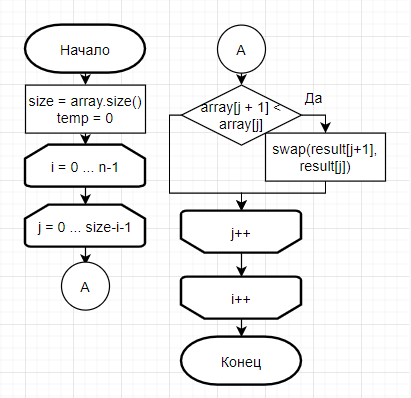
\includegraphics{bubble.png}}
		\caption{Схема алгоритма сортировки пузырьком}
		\label{bubble}
	\end{figure}
	\newpage
	На \hyperref[insert]{рисунке [\ref{insert}]} изображена схема алгоритма сортировки вставками.
	\begin{figure}[h!]
		\center{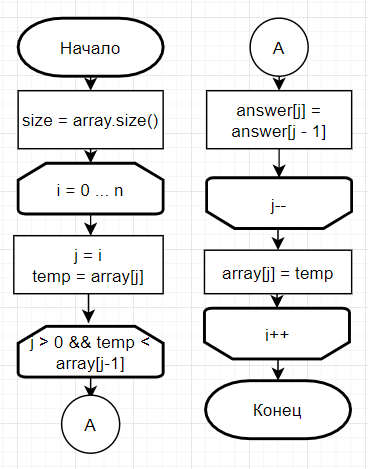
\includegraphics{insert.png}}
		\caption{Схема алгоритма сортировки вставками}
		\label{insert}
	\end{figure}
	\newpage
	На \hyperref[choose]{рисунке  [\ref{choose}]} изображена схема алгоритма сортировки выбором.
	\begin{figure}[h!]
		\center{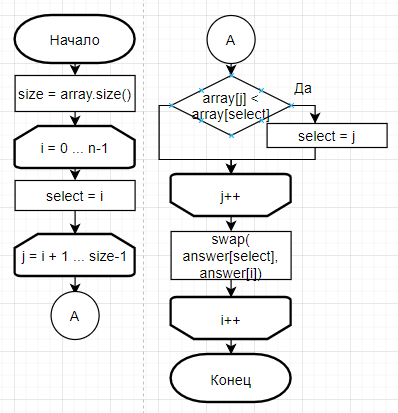
\includegraphics{choose.png}}
		\caption{Схема алгоритма сортировки выбором}
		\label{choose}
	\end{figure}
	\newpage
		 \subsection{Оценка трудоемкости}
		Модель трудоемкости для оценки алгоритмов:
		\newline
		Cтоимость базовых операций единица:
		\newline
		$=,+,*,<,>,<=,>=,==,!=,[],+=,-=,*=,/=,++,--$
		\newline
		\indent 
		\subsubsection{Трудоемкость swap}
	     $f_{swap} = 3 + 4 = 7$
		\subsubsection{Трудоемкость сортировки пузырьком}
		Так как внутренний цикл будет выполняться: $n-0-1,n-1-1,n-2-1,...,n-(n-1)$ раз, то количество выполненных раз можно записать как \hyperref[insBubble]{[\ref{insBubble}]}:
\begin{equation}\label{insBubble}
	int_{bubble}=\frac{(n-1)n}{2}
\end{equation}
	Тогда, если массив отсортирован в обратном порядке, происходит худший случай сортировки пузырьком \hyperref[worstBubble]{[\ref{worstBubble}]}:
	\\
	$
		f_{bubble} = (3 + 1 + (2 + 1 + 2 + 1 + f_{swap}))int_{bubble}) + (2 + 1 + 1)(n - 1)
		 + 1 + 1 = 17int_{bubble} + 4(n - 1) + 2 = \newline
		\frac{17(n-1)n}{2} + 4(n - 1) + 2 \thickapprox \frac{17n^2}{2}
	$\begin{equation}\label{worstBubble}\end{equation}
	А если массив отсортирован, происходит лучший случай \hyperref[bestBubble]{[\ref{bestBubble}]}:
	\begin{equation}\label{bestBubble}
		f_{bubble} = (3 + 1 + (2 + 1 + 1)) int_{bubble}) + (2 + 1 + 1)(n - 1) + 1 + 1 = 8 int_{bubble} + 4(n - 1) + 2 =
		= \frac{8(n-1)n}{2} + 4(n - 1) + 2 \thickapprox 4n^2
	\end{equation}
	

	\subsubsection{Трудоемкость сортировки выбором}
		Так как внутренний цикл будет выполняться: $n-1,n-2,n-3,...,n-(n-1)$ раз, то количество выполненных раз можно записать как \hyperref[insChoose]{[\ref{insChoose}]}:\begin{equation}\label{insChoose}
	int_{choose}=\frac{(n-1)n}{2}
\end{equation}
	Тогда, если массив отсортирован в обратном порядке, происходит худший случай \hyperref[worstChoose]{[\ref{worstChoose}]}:
	\begin{equation}\label{worstChoose}
		f_{choose} = ((2 + 4) * int_{choose}) + (3 + 1 + f_{swap}) * (n - 1) + 2 =
		 \frac{6 * (n-1)n}{2} + 11 * (n - 1) + 2 \thickapprox 3n^2
	\end{equation}
	А если массив отсортирован, происходит лучший случай \hyperref[bestChoose]{[\ref{bestChoose}]}:
	\begin{equation}\label{bestChoose}
		f_{choose} = (2 + 3) * int_{choose}) + (3 + 1 + f_{swap}) * (n - 1) + 2 =
		\frac{5 * (n-1)n}{2} + 11 * (n - 1) + 2 \thickapprox \frac{5n^2}{2}
	\end{equation}


	\subsubsection{Трудоемкость сортировки вставками}
		Так как внутренний цикл будет выполняться: 1, 2, 3, ..., n-1 раз, то количество выполненных раз можно записать как \hyperref[insInsert]{[\ref{insInsert}]}:
\begin{equation}\label{insInsert}
	int_{insert}=\frac{(n-1)n}{2}
\end{equation}
	Тогда, если массив отсортирован в обратном порядке, происходит худший случай \hyperref[worstInsert]{[\ref{worstInsert}]}:
	\begin{equation}\label{worstInsert}
		f_{insert} = ((5 + 5) * int_{insert}) + (2 + 5) * (n - 1) + 2 =
		 \frac{10 * (n-1)n}{2} + 7 * (n - 1) + 2 \thickapprox 5n^2
	\end{equation}
	А если массив отсортирован, происходит лучший случай \hyperref[bestInsert]{[\ref{bestInsert}]}:
	\begin{equation}\label{bestInsert}
		f_{insert} = (2 + 5 + 4) * (n - 1) + 2 = 11 * (n - 1) + 2 \thickapprox 11n
	\end{equation}

	\subsection{Вывод}
	В данном разделе были рассмотрены схемы и была рассчитана трудоемкость алгоритмов и обозначены требования к ПО.
	
	\newpage
	\section{Технологическая часть}
	Ниже будут представлены средствы реализации и листинги реализованной программы.
	\subsection{Средcтва реализации}
	Выбранный язык программирования - С++, так как требований по конкретнему языку не выдвигалось и он был изучен во время обучения. Среда разработки - Visual Studio Code.\cite{vs-code}
	\newline
	\indent Функции вычисления процессорного времени - QueryPerfomanceCounter из библиотеки WinAPI.\cite{winapi}
	
	\subsection{Реализации алгоритмов}
	Ниже представлены листинги реализаций алгоритмов.
	На листинге \hyperref[lstBubble]{[\ref{lstBubble}]} представлен алгоритм сортировки пузырьком.
	\begin{lstlisting}[label=lstBubble, caption=Алгоритм сортировки пузырьком]
	vector<int> sortBubble(vector<int> array)
{
    int size = array.size();
    int temp = 0;
    vector<int> result = array;

    for (int i = 0; i + 1 < size; i++)
    {
        for (int j = 0; j + 1 < size - i; j++)
        {
            if (result[j + 1] < result[j])
            {
                temp = result[j];
                result[j] = result[j + 1];
                result[j + 1] = temp;
            }
        }
    }

    return result;
}
	\end{lstlisting}
		На листинге \hyperref[lstInsertion]{[\ref{lstInsertion}]} Представлен алгоритм сортировки вставками.
	\begin{lstlisting}[label=lstInsertion,caption=Алгоритм сортировки вставками]
	vector<int> sortInsertion(vector<int> array)
{
    int size = array.size();
    int temp = 0;
    vector<int> result = array;

    for (int i = 1; i < size; i++)
    {
        int j = i;
        temp = result[i];
        while (j > 0 && temp < result[j - 1])
        {
            result[j] = result[j - 1];
            j--;
        }
        result[j] = temp;
    }

    return result;
}
	\end{lstlisting}
		На листинге \hyperref[lstSelect]{[\ref{lstSelect}]} Представлен алгоритм сортировки выбором.
	\begin{lstlisting}[label=lstSelect,caption=Алгоритм сортировки выбором]
	vector<int> sortSelect(vector<int> array)
{
    int size = array.size();
    int temp = 0;
    vector<int> result = array;

    for (int i = 0; i < size - 1; i++)
    {
        int select = i;
        for (int j = i + 1; j < size; j++)
        {
            if (result[j] < result[select])
            {
                select = j;
            }
        }
        temp = result[select];
        result[select] = result[i];
        result[i] = temp;
    }

    return result;
}
	\end{lstlisting}

	\subsection{Вывод}
	В данном разделе были описаны средства реализации, были представлены листинги реализации сотрировок пузырьком, вставками и выбором.

	\newpage
	\section{Экспериментальная часть}
	В данной главе будут представлен пример работы программы, результат экспериментов по замеру времени и произведен сравнительный анализ алгоритмов по затрачиваемому времени.
	\subsection{Пример работы программы}
	Пример работы программы представлен на рисунке \hyperref[programmWork]{[\ref{programmWork}]}
	 	\begin{figure}[h!]
		 	\center{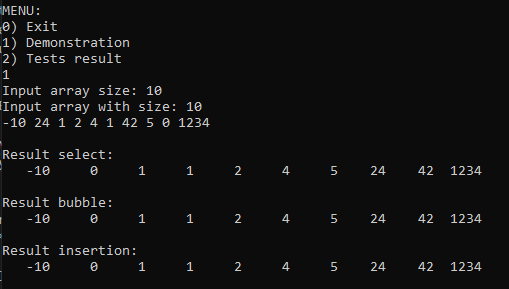
\includegraphics[scale=0.9]{programmWork.png}}
		 	\caption{Пример работы программы}
		 	\label{programmWork}
	 	\end{figure}
	
	\subsection{Сравнительный анализ алгоритмов по времени}
	Эксперименты проводятся на массивах размером от 2 до 252 с шагом 50 (результаты на рисунке \hyperref[resultShort]{[\ref{resultShort}]}
	\begin{figure}[h!]
		 	\center{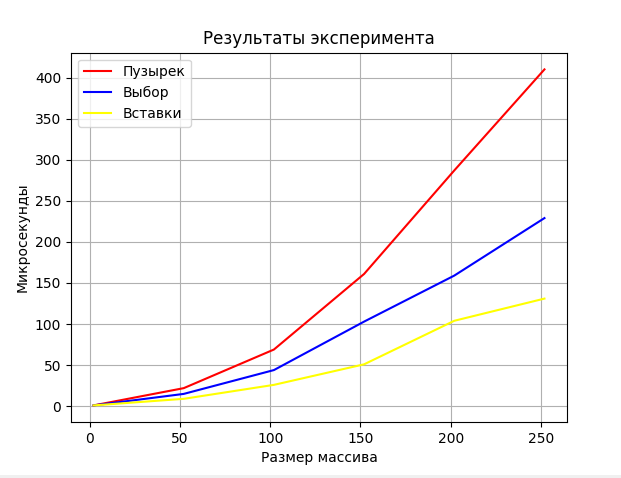
\includegraphics{resultShort.png}}
		 	\caption{Результаты на массивах размером от 2 до 252}
		 	\label{resultShort}
	 	\end{figure}
	\newpage
	\subsection{Вывод}
	Как видно из графиков, самым долгим алгоритмом является алгоритм сортировки пузырьком. 
	Самым быстрым является алгоритм сортировки вставками. Алгоритм сортировки выбором быстрее 
	сортировки пузырьком, но уступает в скорости работы алгоритму сортировки вставками.

	\newpage
	\begin{center}
		\section*{Заключение}
	\end{center}
	\addcontentsline{toc}{section}{Заключение}
	\indent \indent В данной лабораторной работе были описаны алгоритмы сортировки пузырьком, вставками и выбором, они были реализованы, а также были проведены эксперименты по замеру времени работы реализованных алгоритмов и проведены сравнения алгоритмов по результатам эксперимента. Также была дана оценка трудоемкости.
	\newpage
	\addcontentsline{toc}{section}{Список литературы}
	
	\begin{center}
	\begin{thebibliography}{3}
	\bibitem{baseSort}
	Базовые сортировки [Электронный ресурс]. Режим доступа: (дата обращения - 02.10.2020) Свободный. URL:https://tproger.ru/translations/sorting-for-beginners/
	\bibitem{vs-code}
	Visual Studio Code [Электронный ресурс]. Режим доступа: (дата обращения - 02.10.2020) Свободный. URL: code.visualstudio.com
	\bibitem{winapi}
		WinAPI. Функция QueryPerformanceCounter [Электронный ресурс]. Режим доступа: (дата обращения - 02.10.2020) Свободный. URL: https://docs.microsoft.com/en-us/windows/win32/api/profileapi/nf-profileapi-queryperformancecounter
	\end{thebibliography}
	\end{center}
\end{document}